% ============================================================
% M3 S3 练习件·W3 臂G 片1 —— 课时18 2.8②压轴综合二＝照抄课时01 母版体例
% 生成：M3 成卷轮 S3 W3 臂G｜2026-09-14｜编译 cwd＝本目录（中文路径禁 \input 绝对路径）
%   xelatex main-true.tex ×2 → 含详解印本；xelatex main-false.tex ×2 → 纯题版（单源双本）
% 输入链（全只读）：题面库 课时18-2.8②压轴综合二.md（题面逐字装配）＋ -答案侧.md（值逐字回嵌）
%   ＋ 定稿/批E-课时18-2.8②压轴综合二.md §七 补产全文区（详解回嵌源）；toolchain＝qp-m3.sty
%   （钉后版 md5 7c3930362be8a0a2bdf21bbf8ac16573，本地挂载副本，破损即停）。
% 母版体例：详见《练习件母版体例说明.md》（课时01）；同波近范模：课时12（W3 臂F 片1）；
%   门谱读数见 过程件 工作区/_tmpM3S3W3臂G0914/。
% 键账：件内 ansblock 键集 ≡ 题面库片练键集 ≡ manifest 练键序 01~16（16 键，零缺漏零多余）；
%   拓区隔离：2章-拓/测/滚 键不入本件（S4 拓展册收）；导学键 2章-导-课时18-G1~G5 属导学件域，
%   亦不入（G1 0914 撤换回冲 3章件17-#19 在案，撤换系导学席，练习键序/值零涉）。
% 卷式例外案B：练习件不属卷式——答案块物理落点恒为题后 ansblock，禁卷末附卷制；
%   全线括线模（导言 \ansblockgrayfalse 一次置定，件内不切换；灰底盒不可跨栏断，练习件禁用）。
% 题序＝manifest 键序 01~16（零重排）；印面题号 1~16 连号（\tihao 号＝\ansitem 号同键）；
%   三档切位 1~7／8~14／15~16（照库序切位，非难度重排；本片 0 简，压轴域素材域事实，
%   批E-台账 §五.10 在案）。
% 槽配实录：单选2（01/10）＋多选1（02，≤4 合规）＋填空0＋解答13（03~09/11~16）；
%   10选4填2解 为波次方案基线槽配，本片实配照题面侧头标（批E §一 满足度同口径：2.8② 压轴
%   课位解答超配、选择欠配按实登记，不硬凑）。
% 选项槽位：默认四连排（0.25\linewidth−0.25\lxhang），超宽降档梯 四连排→两连排
%   （0.5\linewidth−0.5\lxhang−0.25em）→单列 \lxopt；禁缩字号/负 kern/删标点凑宽。
%   本片实测降档：题1 四连排、题2 单列、题10 两连排（真算读数见 值台账-课时18.json「降档登记」）。
% 解答书写区：E 位 03~09/11~16 十三题均两问，\liubai[24mm]{解答书写区}（两问档；
%   16~40mm 带内；纯题档吞 ansblock 不吞 \liubai）。
% 填空印答：本片填空 0，\kongda 计数＝0。
% 图债：题12(2)（18-12）「如图」构形图、题14（18-14）拼接曲线图已于 0914 印前回冲印面
%   （图资源/18-12.png、18-14.png，卷②/富矿件提取；题面「如图」处 \ansfig 插桩；
%   台账「图债」字段同账销案）。
% 题面注记（不入印面）：18-03/05/08/09 主载体 x²/4+y²/3=1 共4题（前置闸0913 黄旗③，同卷
%   装配注意分散）；18-04 源(2)数值系亲算补出（⑤-5，不得标「见源解析」）；18-09 定点亲算
%   补出（⑤-5）；18-13 指纹 P(−2,1)≠源文 P(−2,0)，以源文为准（§三.3）；18-16 定点措辞按
%   亲算⑤-4 钉死口径作「与」（两点同时在圆上）。
% ============================================================
\documentclass[fontset=none]{ctexart}
\usepackage{qp-m3}
% —— 印面逐字符号路由补钉（承导学件母版；− 走 TNR、▱ NSC 子块；禁改 sty 保 md5） ——
\xeCJKDeclareCharClass{Default}{"2212}%
\setCJKfamilyfont{nscblk}[Path=C:/提示词/工作区/字替对照-0909/variantF/fonts/,BoldFont=NSC-w600.ttf]{NSC-w500.ttf}%
\xeCJKDeclareSubCJKBlock{nscblk}{"25B1}%
\newcommand{\pxparallelogram}{{\CJKfamily{nscblk}▱}}%
% —— 文本态下划线安全（18-03 值 S_max 直印；数学态仍下标；内核方案，不引包） ——
\begingroup
  \catcode`\_=13 %
  \gdef_{\TextOrMath{\textunderscore}{\sb}}%
\endgroup
\AtBeginDocument{\catcode`\_=13 }%
% —— 断行微调（CJK 胶 0.10em＋拉伸 plus 0.30em，课时16 实证校准 0914：窄栏详解长公式链；
%    \emergencystretch 不另设） ——
\xeCJKsetup{CJKglue={\hskip 0.10em plus 0.30em minus 0.05em}}%
% —— 练习件全线括线模（S3 波次方案 §四.3：导言一次置定、件内不切换） ——
\ansblockgrayfalse
% —— 页脚件名（qp-headfoot 复用入口） ——
\renewcommand{\qpzhangming}{第二章\quad 平面解析几何}%
\renewcommand{\qpjianming}{练习件}%

\begin{document}
%装配轮S6三本跨本连续页码（G7方案B）setcounter 注入位
\setcounter{page}{235}

\keshi{第18课时\quad 2.8② 压轴综合（二）}
\begin{multicols}{2}
\emergencystretch=1em

% ============================================================
% 基础巩固（题1~7＝18-01~07：单选1＋多选1＋解答5；题后紧跟答案制，全线括线 ansblock）
% ============================================================
\dangbadge{基}{础}{巩}{固}

\tihao{1}\zu{向量平行定比×单选} \tieside{中档(知识点二)}设双曲线\(E\)：\(x^{2}-y^{2}/3=1\)的左、右焦点为\(F_1\)、\(F_2\)，左顶点为\(A\)，点\(M\)是双曲线\(E\)在第一象限内的一点，直线\(MF_1\)交双曲线\(E\)的左支于点\(N\)，若\(NA\parallel MF_2\)，则\(|MF_2|=\)\nobreak(\kongwei)
\bindopt {\fontsize{10.5pt}{\qpTJgLeadLiti}\selectfont \makebox[\dimexpr0.25\linewidth-0.25\lxhang\relax][l]{A．\(7/4\)}\makebox[\dimexpr0.25\linewidth-0.25\lxhang\relax][l]{B．\(5/2\)}\makebox[\dimexpr0.25\linewidth-0.25\lxhang\relax][l]{C．\(8/3\)}\makebox[\dimexpr0.25\linewidth-0.25\lxhang\relax][l]{D．\(11/4\)}\par}

\begin{ansblock}[2章-练-课时18-01]
% ans:2章-练-课时18-01
\ansitem{1}{B（|MF₂|=5/2）}
\ansnote{详解}{\(F_1(-2,0)\)、\(F_2(2,0)\)、\(A(-1,0)\)，故\(|F_1A|/|F_1F_2|=1/4\)。\par\noindent \(NA\parallel MF_2\Rightarrow\hskip 0pt plus 1em\relax \triangle F_1AN\sim \triangle F_1MF_2\Rightarrow\hskip 0pt plus 1em\relax F_1N/F_1M=1/4\)。设\(M(x_0,y_0)\)（\(x_0>0\)，\(y_0>0\)），则\(N=F_1+(1/4)(M-F_1)=((x_0-6)/4,y_0/4)\)。\(M\)、\(N\)均在\(E\)上：\(x_0^{2}-y_0^{2}/3=1\)且\(((x_0-6)/4)^{2}-(y_0/4)^{2}/3=1\)，后者乘16得\((x_0-6)^{2}-y_0^{2}/3=16\)；两式相减\((x_0-6)^{2}-x_0^{2}=15\)，即\(-12x_0+36=15\)，得\(x_0=7/4\)，进而\(y_0^{2}=3(x_0^{2}-1)=99/16\)，\(y_0=3\sqrt{11}/4\)。于是\(|MF_2|=\sqrt{(7/4-2)^{2}+99/16}=\sqrt{100/16}=5/2\)。故选：B。}
\end{ansblock}

\tihao{2}\duoxuan\hspace{0.6em}\zu{多选结论判定×多选} \tieside{中档(知识点一)}已知抛物线\(C\)：\(y^{2}=8x\)，\(O\)为坐标原点，其焦点为\(F\)，准线与\(x\)轴相交于\(M\)点，经过\(M\)点且斜率为\(k\)的直线\(l\)与抛物线相交于\(A(x_1,y_1)\)、\(B(x_2,y_2)\)两点，则下列结论中正确的是\nobreak(\kongwei)

\lxopt{A．\(-1<k<1\)}

\lxopt{B．\(y_1y_2=8x_1x_2\)}

\lxopt{C．\(\angle AFB\)可能为直角}

\lxopt{D．当\(k^{2}=1/2\)时，\(\triangle AFB\)的面积为16}

\begin{ansblock}[2章-练-课时18-02]
% ans:2章-练-课时18-02
\ansitem{2}{CD}
\ansnote{详解}{\(F(2,0)\)，准线\(x=-2\)，即\(M(-2,0)\)，\(l\)：\(y=k(x+2)\)。联立得\(k^{2}x^{2}+(4k^{2}-8)x+4k^{2}=0\)；由两交点得\(k^{2}\neq 0\)且\(\Delta=64(1-k^{2})>0\)，即\(-1<k<1\)且\(k\neq 0\)——A漏\(k\neq 0\)，错。改以\(y\)为主元：\(x=y^{2}/8\)代入\(l\)得\(ky^{2}-8y+16k=0\)，故\(y_1+y_2=8/k\)、\(y_1y_2=16\)；而\(x_1x_2=4\)，即\(8x_1x_2=32\neq 16\)，B错。\par\noindent \(\overrightarrow{FA}\cdot\overrightarrow{FB}=(x_1-2)(x_2-2)+y_1y_2=x_1x_2-2(x_1+x_2)+4+y_1y_2\)，其中\(x_1+x_2=(8-4k^{2})/k^{2}\)，代入得\(\overrightarrow{FA}\cdot\overrightarrow{FB}=32-16/k^{2}\)，当\(k^{2}=1/2\)时为0，即\(\angle AFB\)可为直角，C对。\(S=(1/2)|MF|\cdot|y_1-y_2|=2\sqrt{(y_1+y_2)^{2}-4y_1y_2}=2\sqrt{64/k^{2}-64}\)；\(k^{2}=1/2\)时\(|y_1-y_2|=8\)，即\(S=16\)，D对。故选：CD。}
\end{ansblock}

\tihao{3}\zu{向量垂直→面积最值×解答} \tieside{难(知识点三)}设抛物线\(y^{2}=2px\)（\(p>0\)）的焦点为\(F\)，点\(F\)到抛物线准线的距离为2。若椭圆\(x^{2}/a^{2}+y^{2}/b^{2}=1\)（\(a>b>0\)）的右焦点也为\(F\)，离心率为\(1/2\)。(1) 求抛物线方程和椭圆方程；(2) 若不经过\(F\)的直线\(l\)与抛物线交于\(A\)、\(B\)两点，且\(\overrightarrow{OA}\cdot\overrightarrow{OB}=-3\)（\(O\)为坐标原点），直线\(l\)与椭圆交于\(C\)、\(D\)两点，求\(\triangle CDF\)面积的最大值。
\liubai[24mm]{解答书写区}

\begin{ansblock}[2章-练-课时18-03]
% ans:2章-练-课时18-03
\ansitem{3}{(1) y²=4x、x²/4+y²/3=1；(2) S_max=2√3/3}
\ansnote{详解}{(1) 焦点到准线距离\(p=2\)，即\(y^{2}=4x\)，\(F(1,0)\)；椭圆\(c=1\)、\(e=c/a=1/2\)，即\(a=2\)、\(b^{2}=a^{2}-c^{2}=3\)，故\(x^{2}/4+y^{2}/3=1\)。\par\noindent (2) 设\(l\)：\(x=my+n\)（不过\(F\)，即\(n\neq 1\)）。交抛物线：\(y^{2}-4my-4n=0\)，得\(y_1y_2=-4n\)、\(x_1x_2=(y_1y_2)^{2}/16=n^{2}\)。\(\overrightarrow{OA}\cdot\overrightarrow{OB}=n^{2}-4n=-3\)，得\(n=1\)（此时\(l\)过\(F(1,0)\)，舍）或\(n=3\)。交椭圆：\(3(my+3)^{2}+4y^{2}=12\)，即\((3m^{2}+4)y^{2}+18my+15=0\)，\(\Delta=144m^{2}-240\geqslant 0\)，即\(m^{2}\geqslant 5/3\)。\par\noindent \(l\)交\(x\)轴于\(T(3,0)\)，\(|TF|=2\)，故\(S=|y_C-y_D|\)，\(S^{2}=(144m^{2}-240)/(3m^{2}+4)^{2}\)。令\(u=3m^{2}+4\)（\(u\geqslant 9\)）：\(S^{2}=48/u-432/u^{2}\)；再令\(v=1/u\in(0,1/9]\)：\(S^{2}=48v-432v^{2}\)在\(v=1/18\)处取最大（\(1/18\in(0,1/9]\)），\(S^{2}\)的最大值为\(48/18-432/324=4/3\)，即\(S_{max}=2\sqrt{3}/3\)，此时\(3m^{2}+4=18\)，\(m^{2}=14/3\)，满足\(m^{2}\geqslant 5/3\)。}
\end{ansblock}

\tihao{4}\zu{向量垂直→面积定值×解答} \tieside{难(知识点三)}已知椭圆\(x^{2}+2y^{2}=1\)，过原点的两条直线\(l_1\)和\(l_2\)分别与椭圆交于\(A\)、\(B\)和\(C\)、\(D\)，记得到的平行四边形\(ACBD\)的面积为\(S\)。(1) 设\(A(x_1,y_1)\)、\(C(x_2,y_2)\)，用\(A\)、\(C\)的坐标表示点\(C\)到直线\(l_1\)的距离，并证明\(S=2|x_1y_2-x_2y_1|\)；(2) 从①②两个问题中任选一个作答：①设\(l_1\)与\(l_2\)的斜率之积为\(-1/2\)，求面积\(S\)的值；②设\(l_1\)与\(l_2\)的斜率之积为\(m\)，求\(m\)的值，使得无论\(l_1\)与\(l_2\)如何变动，面积\(S\)保持不变。
\liubai[24mm]{解答书写区}

\begin{ansblock}[2章-练-课时18-04]
% ans:2章-练-课时18-04
\ansitem{4}{(1) d=|x₁y₂−x₂y₁|/√(x₁²+y₁²)，证毕；①S=√2；②m=−1/2（此时 S≡√2）}
\ansnote{详解}{(1) \(l_1\)：\(y_1x-x_1y=0\)（\(x_1=0\)时即\(x=0\)，公式仍适用），故\(d=|y_1x_2-x_1y_2|/\sqrt{x_1^{2}+y_1^{2}}\)。\(O\)同时平分\(AB\)与\(CD\)，故\(S=4S_{\triangle OAC}=4\cdot(1/2)|OA|\cdot d=2\sqrt{x_1^{2}+y_1^{2}}\cdot|x_1y_2-x_2y_1|/\sqrt{x_1^{2}+y_1^{2}}=2|x_1y_2-x_2y_1|\)，证毕。\par\noindent (2) 记\(y_i=k_ix_i\)，则\(x_i^{2}=1/(1+2k_i^{2})\)，\(S=2|x_1||x_2||k_2-k_1|=2|k_2-k_1|/\sqrt{(1+2k_1^{2})(1+2k_2^{2})}\)。\par\noindent ①\(k_1k_2=-1/2\)：分母\(=(1+2k_1^{2})(1+2k_2^{2})=1+2(k_1^{2}+k_2^{2})+4k_1^{2}k_2^{2}=2(1+k_1^{2}+k_2^{2})\)；又\((k_2-k_1)^{2}=k_1^{2}+k_2^{2}-2k_1k_2=1+k_1^{2}+k_2^{2}\)，故\(S^{2}=4(1+k_1^{2}+k_2^{2})/[2(1+k_1^{2}+k_2^{2})]=2\)，即\(S=\sqrt{2}\)。\par\noindent ②记\(T=k_1^{2}+k_2^{2}\)，则\((k_2-k_1)^{2}=T-2m\)、分母\(=2T+1+4m^{2}\)，\(S^{2}=4(T-2m)/(2T+1+4m^{2})\)。要与\(T\)无关，须存在\(\lambda\)使\(T-2m\equiv \lambda(2T+1+4m^{2})\)：比较系数\(2\lambda=1\)、\(\lambda(1+4m^{2})=-2m\)，即\((1+4m^{2})/2=-2m\)，\(4m^{2}+4m+1=0\)，得\(m=-1/2\)（与①自洽，此时对一切\(T\)有\(S^{2}=2\)）。}
\end{ansblock}
\tihao{5}\zu{定值求参×解答} \tieside{中档(知识点三)}已知抛物线\(G\)：\(y^{2}=4x\)的焦点与椭圆\(E\)：\(x^{2}/a^{2}+y^{2}/b^{2}=1\)（\(a>b>0\)）的右焦点\(F\)重合，椭圆\(E\)的长轴长为4。(1) 求椭圆\(E\)的方程；(2) 过点\(F\)且斜率为\(k\)的直线\(l\)交椭圆\(E\)于\(A\)、\(B\)两点，交抛物线\(G\)于\(M\)、\(N\)两点，请问是否存在实常数\(t\)，使\(2/|AB|+t/|MN|\)为定值？若存在，求出\(t\)的值；若不存在，说明理由。
\liubai[24mm]{解答书写区}

\begin{ansblock}[2章-练-课时18-05]
% ans:2章-练-课时18-05
\ansitem{5}{(1) x²/4+y²/3=1；(2) 存在，t=−2/3，定值 1/2}
\ansnote{详解}{(1) \(y^{2}=4x\)焦点\((1,0)\)，即\(c=1\)；长轴\(2a=4\)，即\(a=2\)、\(b^{2}=3\)，故\(x^{2}/4+y^{2}/3=1\)。\par\noindent (2) \(l\)：\(y=k(x-1)\)（\(k\neq 0\)）。交椭圆：\((3+4k^{2})x^{2}-8k^{2}x+4k^{2}-12=0\)，\(|AB|=\sqrt{1+k^{2}}\cdot\sqrt{(x_1+x_2)^{2}-4x_1x_2}=12(1+k^{2})/(3+4k^{2})\)。交抛物线：\(k^{2}x^{2}-(2k^{2}+4)x+k^{2}=0\)，\(x_3+x_4=(2k^{2}+4)/k^{2}\)，\(|MN|=x_3+x_4+2=4(1+k^{2})/k^{2}\)（焦点弦）。于是\(2/|AB|+t/|MN|=(3+4k^{2})/(6(1+k^{2}))+tk^{2}/(4(1+k^{2}))=[(8+3t)k^{2}+6]/(12(1+k^{2}))\)，与\(k\)无关当且仅当\(8+3t=6\)，即\(t=-2/3\)，此时定值\(=6/12=1/2\)。}
\end{ansblock}

\tihao{6}\zu{定值辨析×解答} \tieside{中档(知识点三)}已知抛物线\(C\)：\(y^{2}=-4x\)，直线\(l\)过定点\(P(0,1)\)。(1) 若\(l\)与\(C\)仅有一个公共点，求直线\(l\)的方程；(2) 若\(l\)与\(C\)交于\(A\)、\(B\)两点，直线\(OA\)、\(OB\)（\(O\)为坐标原点）的斜率分别为\(k_1\)、\(k_2\)，试探究在\(k_1-k_2\)、\(k_1+k_2\)、\(k_1/k_2\)、\(k_1k_2\)中，运算结果是否为定值？并说明理由。
\liubai[24mm]{解答书写区}

\begin{ansblock}[2章-练-课时18-06]
% ans:2章-练-课时18-06
\ansitem{6}{(1) y=1 或 x=0 或 y=−x+1；(2) 仅 k₁+k₂=−4 为定值，其余三个均不是}
\ansnote{详解}{(1) 分三类：与对称轴（\(x\)轴）平行的直线\(y=1\)，恰一公共点；过顶点的切线\(x=0\)；斜线\(y=kx+1\)（\(k\neq 0\)）代入得\(k^{2}x^{2}+(2k+4)x+1=0\)，令\(\Delta=(2k+4)^{2}-4k^{2}=16k+16=0\)，得\(k=-1\)，即\(y=-x+1\)。共三条。\par\noindent (2) 有两交点，即\(k\)存在、\(k\neq 0\)且\(\Delta=16k+16>0\)，即\(k>-1\)。联立\(k^{2}x^{2}+(2k+4)x+1=0\)，得\(x_1+x_2=-(2k+4)/k^{2}\)、\(x_1x_2=1/k^{2}\)。\(k_i=y_i/x_i=k+1/x_i\)：\(k_1+k_2=2k+(x_1+x_2)/(x_1x_2)=2k-(2k+4)=-4\)，为定值。\(k_1k_2=y_1y_2/(x_1x_2)\)，而\(y_1y_2=(kx_1+1)(kx_2+1)=k^{2}x_1x_2+k(x_1+x_2)+1=-4/k\)，故\(k_1k_2=-4k\)，随\(k\)变；\(|k_1-k_2|=|x_2-x_1|/|x_1x_2|=4\sqrt{k+1}\)（\(|x_1-x_2|=\sqrt{(x_1+x_2)^{2}-4x_1x_2}=4\sqrt{k+1}/k^{2}\)）随\(k\)变；\(k_1/k_2\)同理随\(k\)变。故仅\(k_1+k_2=-4\)为定值。}
\end{ansblock}

\tihao{7}\zu{定点存在性（等差椭圆）×解答} \tieside{中档(知识点二)}焦距为\(2c\)的椭圆\(\Gamma\)：\(x^{2}/a^{2}+y^{2}/b^{2}=1\)（\(a>b>0\)），如果满足「\(2b=a+c\)」，则称此椭圆为「等差椭圆」。(1) 如果椭圆\(\Gamma\)是「等差椭圆」，求\(b/a\)的值；(2) 对于焦距为12的「等差椭圆」，点\(A\)为椭圆短轴的上顶点，\(P\)为椭圆上异于\(A\)点的任一点，\(Q\)为\(P\)关于原点\(O\)的对称点（\(Q\)也异于\(A\)），直线\(AP\)、\(AQ\)分别与\(x\)轴交于\(M\)、\(N\)两点，判断以线段\(MN\)为直径的圆是否过定点？说明理由。
\liubai[24mm]{解答书写区}

\begin{ansblock}[2章-练-课时18-07]
% ans:2章-练-课时18-07
\ansitem{7}{(1) 4/5；(2) 恒过定点 (0,±10)}
\ansnote{详解}{(1) \(2b=a+c\)，即\(c=2b-a\)，代入\(c^{2}=a^{2}-b^{2}\)：\((2b-a)^{2}=a^{2}-b^{2}\)，即\(4b^{2}-4ab=0\)，故\(b/a=4/5\)。\par\noindent (2) \(2c=12\)，即\(c=6\)；\(b^{2}=16a^{2}/25\)配\(a^{2}-b^{2}=36\)，得\(9a^{2}/25=36\)，即\(a^{2}=100\)、\(b^{2}=64\)，\(A(0,8)\)。设\(P(x_0,y_0)\)（\(x_0\neq 0\)），\(Q(-x_0,-y_0)\)。直线\(AP\)：\(y=(y_0-8)x/x_0+8\)，令\(y=0\)，得\(M(8x_0/(8-y_0),0)\)；同理\(N(-8x_0/(8+y_0),0)\)。\par\noindent 以\(MN\)为直径的圆：\((x-8x_0/(8-y_0))(x+8x_0/(8+y_0))+y^{2}=0\)，其中交叉项\(=8x_0[(8-y_0-(8+y_0))/(64-y_0^{2})]=-16x_0y_0/(64-y_0^{2})\)。由\(x_0^{2}/100+y_0^{2}/64=1\)得\(64-y_0^{2}=64x_0^{2}/100=16x_0^{2}/25\)，故圆方程化为\(x^{2}+y^{2}-(25y_0/x_0)x-100=0\)。令\(x=0\)得\(y=\pm 10\)，与\(P\)无关，即恒过定点\((0,10)\)与\((0,-10)\)（\(P\)异于\(A\)保证\(x_0\neq 0\)、\(64-y_0^{2}>0\)）。}
\end{ansblock}

% ============================================================
% 综合提升（题8~14＝18-08~14：解答7＋单选1（题10 照库序居本档）；书写区 \liubai[24mm]（两问档）
%   ＋题后括线 ansblock）
% ============================================================
\dangbadge{综}{合}{提}{升}

\tihao{8}\zu{定点存在性（轨迹＋角等）×解答} \tieside{中档(知识点二)}已知圆\(A\)：\(x^{2}+y^{2}+2x-15=0\)和定点\(B(1,0)\)，\(M\)是圆\(A\)上任意一点，线段\(MB\)的垂直平分线交\(MA\)于点\(N\)，设点\(N\)的轨迹为\(C\)。(1) 求\(C\)的方程；(2) 若直线\(y=k(x-1)\)与曲线\(C\)相交于\(P\)、\(Q\)两点，试问：在\(x\)轴上是否存在定点\(R\)，使当\(k\)变化时，总有\(\angle ORP=\angle ORQ\)？若存在，求出点\(R\)的坐标；若不存在，请说明理由。
\liubai[24mm]{解答书写区}

\begin{ansblock}[2章-练-课时18-08]
% ans:2章-练-课时18-08
\ansitem{8}{(1) x²/4+y²/3=1；(2) 存在，R(4,0)}
\ansnote{详解}{(1) 圆\(A\)即\((x+1)^{2}+y^{2}=16\)，圆心\(A(-1,0)\)、半径4。由垂直平分线，\(|NM|=|NB|\)，而\(N\)在\(MA\)上，故\(|NA|+|NB|=|NA|+|NM|=|MA|=4>|AB|=2\)，轨迹为以\(A\)、\(B\)为焦点的椭圆：\(2a=4\)、\(2c=2\)，\(a^{2}=4\)、\(b^{2}=3\)，即\(x^{2}/4+y^{2}/3=1\)。\par\noindent (2) 设\(R(t,0)\)。联立\((4k^{2}+3)x^{2}-8k^{2}x+4k^{2}-12=0\)，得\(x_1+x_2=8k^{2}/(4k^{2}+3)\)、\(x_1x_2=(4k^{2}-12)/(4k^{2}+3)\)。\(\angle ORP=\angle ORQ\)当且仅当\(k_{RP}+k_{RQ}=0\)，即\(y_1/(x_1-t)+y_2/(x_2-t)=0\)。以\(y_i=k(x_i-1)\)代入，分子\(=k[2x_1x_2-(1+t)(x_1+x_2)+2t]=0\)；\(k\neq 0\)时即\(2(4k^{2}-12)-8k^{2}(1+t)+2t(4k^{2}+3)=0\)，展开\(8k^{2}-24-8k^{2}-8k^{2}t+8k^{2}t+6t=0\)，即\(6t-24=0\)，得\(t=4\)（\(k=0\)时\(P\)、\(Q\)为长轴两端点，等式显然）。故存在\(R(4,0)\)，与\(k\)无关。}
\end{ansblock}

\tihao{9}\zu{条件选择×解答} \tieside{难(知识点二)}在平面直角坐标系\(xOy\)中，已知椭圆\(C\)：\(x^{2}/a^{2}+y^{2}/b^{2}=1\)（\(a>b>0\)），\(F\)是椭圆的右焦点且\kongbai{}，从下列条件中任选一个补充在上面问题中并作答（注：如果选择多个条件作答，按第一个计分）。条件①：椭圆\(C\)的离心率\(e=1/2\)，焦点到相应准线的距离是3；条件②：椭圆\(C\)与圆\(M\)：\((x-6)^{2}+y^{2}=16\)外切，又与圆\(N\)：\(x^{2}+(y-2\sqrt{3})^{2}=3\)外切。(1) 求椭圆\(C\)的方程；(2) 已知\(A\)、\(B\)是椭圆\(C\)上关于原点对称的两点，\(A\)在\(x\)轴的上方，连接\(AF\)、\(BF\)并分别延长交椭圆\(C\)于\(D\)、\(E\)两点，证明：直线\(DE\)过定点。
\liubai[24mm]{解答书写区}

\begin{ansblock}[2章-练-课时18-09]
% ans:2章-练-课时18-09
\ansitem{9}{(1) 两条件均得 x²/4+y²/3=1；(2) DE 恒过定点 (8/5,0)}
\ansnote{详解}{(1) 条件①：\(e=1/2\)，即\(a=2c\)；\(a^{2}/c-c=3\)，即\(4c-c=3\)，得\(c=1\)，\(a^{2}=4\)、\(b^{2}=3\)。条件②：圆\(M\)圆心\((6,0)\)、半径4，椭圆在圆内一侧外切，切点必为右顶点，即\(a+4=6\)，得\(a=2\)；圆\(N\)圆心\((0,2\sqrt{3})\)、半径\(\sqrt{3}\)，得\(b=\sqrt{3}\)、\(b^{2}=3\)。回验唯一性（外切即恰一公共点）：圆\(M\)与椭圆联立消\(y\)得\(x^{2}-48x+92=0\)，\(x=2\)或46（46越界舍）；圆\(N\)联立得\(y^{2}+12\sqrt{3}y-39=0\)，\(y=\sqrt{3}\)或\(-13\sqrt{3}\)（越界舍）。两条件同得\(x^{2}/4+y^{2}/3=1\)。\par\noindent (2) \(F(1,0)\)。设\(A(x_1,y_1)\)（\(y_1>0\)）、\(B(-x_1,-y_1)\)，满足\(3x_1^{2}+4y_1^{2}=12\)。直线\(AF\)：\(x=my+1\)（\(m=(x_1-1)/y_1\)）、直线\(BF\)：\(x=ny+1\)（\(n=(x_1+1)/y_1\)），\(n-m=2/y_1\)。\(x=my+1\)代入\(3x^{2}+4y^{2}=12\)：\((3m^{2}+4)y^{2}+6my-9=0\)，得\(y_1y_D=-9/(3m^{2}+4)\)，即\(y_D=-9/[(3m^{2}+4)y_1]\)；同理以\(-y_1\)为一根，得\(y_E=9/[(3n^{2}+4)y_1]\)，且\(x_D=my_D+1\)、\(x_E=ny_E+1\)。\par\noindent \(D\)、\(E\)、\(P(8/5,0)\)共线当且仅当\(y_D(x_E-8/5)=y_E(x_D-8/5)\)，即\(y_Dy_E(n-m)=(3/5)(y_D-y_E)\)（\(*\)）。代入\(y_Dy_E=-81/[(3m^{2}+4)(3n^{2}+4)y_1^{2}]\)、\(y_D-y_E=-(9/y_1)(3m^{2}+3n^{2}+8)/[(3m^{2}+4)(3n^{2}+4)]\)，则（\(*\)）等价于\(30/y_1^{2}=3(m^{2}+n^{2})+8\)，即\(30=3y_1^{2}(m^{2}+n^{2})+8y_1^{2}=3[(x_1-1)^{2}+(x_1+1)^{2}]+8y_1^{2}=6x_1^{2}+6+8y_1^{2}=2(3x_1^{2}+4y_1^{2})+6=24+6=30\)，恒成立。故\(DE\)恒过定点\((8/5,0)\)（另以\(A(0,\sqrt{3})\)、\(A(6/5,4\sqrt{3}/5)\)两例回验\(DE\)与\(x\)轴交点同为\(8/5\)）。}
\end{ansblock}
\tihao{10}\zu{存在性计数定参×单选} \tieside{中档(知识点二)}过双曲线\(x^{2}/a^{2}-y^{2}/3=1\)（\(a>0\)）的右焦点\(F\)作直线\(l\)与双曲线交于\(A\)、\(B\)两点，使得\(|AB|=6\)，若这样的直线有且只有两条，则实数\(a\)的取值范围是\nobreak(\kongwei)
\bindopt {\fontsize{10.5pt}{\qpTJgLeadLiti}\selectfont \makebox[\dimexpr0.5\linewidth-0.5\lxhang-0.25em\relax][l]{A．\((0,1]\cup(3,+\infty)\)}\makebox[\dimexpr0.5\linewidth-0.5\lxhang-0.25em\relax][l]{B．\((0,1)\cup(3,+\infty)\)}\par}
\bindopt {\fontsize{10.5pt}{\qpTJgLeadLiti}\selectfont \makebox[\dimexpr0.5\linewidth-0.5\lxhang-0.25em\relax][l]{C．\((0,1)\)}\makebox[\dimexpr0.5\linewidth-0.5\lxhang-0.25em\relax][l]{D．\((3,+\infty)\)}\par}

\begin{ansblock}[2章-练-课时18-10]
% ans:2章-练-课时18-10
\ansitem{10}{B}
\ansnote{详解}{过焦点的弦分两型：跨支型（\(A\)、\(B\)各在一支）弦长下限为\(2a\)，且实轴所在直线（长\(2a\)）恰1条，长\(L>2a\)时对称地有2条；单支型（同在右支）弦长下限为通径\(2b^{2}/a=6/a\)，通径（\(l\perp x\)轴）恰1条，\(L>6/a\)时有2条。且\(6/a\)与\(2a\)不可能同时等于6（\(a=1\)时\(6/a=6\)、\(2a=2\)；\(a=3\)时\(2a=6\)、\(6/a=2\)）。令\(L=6\)分段计数：\par\noindent \(a<1\)：跨支\(6>2a\)，有2条，单支\(6<6/a\)，有0条，合计2；\par\noindent \(a=1\)：\(2+1=3\)；\(1<a<3\)：\(2+2=4\)；\(a=3\)：\(1+2=3\)，均不合；\par\noindent \(a>3\)：跨支\(6<2a\)，有0条，单支\(6>6/a\)，有2条，合计2。\par\noindent 故\(a\in(0,1)\cup(3,+\infty)\)，选：B。}
\end{ansblock}

\tihao{11}\zu{存在性否定×解答} \tieside{难(知识点二)}已知椭圆\(C\)：\(x^{2}/a^{2}+y^{2}/b^{2}=1\)（\(a>b>0\)）的离心率为\(\sqrt{2}/2\)，椭圆的右焦点与右顶点及上顶点构成的三角形面积为\(\sqrt{2}-1\)。(1) 求椭圆\(C\)的标准方程；(2) 已知直线\(y=k(x-1)\)与椭圆\(C\)交于\(A\)、\(B\)两点，若点\(Q\)的坐标为\((7/4,0)\)，问：是否存在\(k\)，使得\(\overrightarrow{QA}\cdot\overrightarrow{QB}>1\)？若存在，求出\(k\)的取值范围；不存在，请说明理由。
\liubai[24mm]{解答书写区}

\begin{ansblock}[2章-练-课时18-11]
% ans:2章-练-课时18-11
\ansitem{11}{(1) x²/4+y²/2=1；(2) 不存在（QA·QB≡−15/16 恒<1）}
\ansnote{详解}{(1) \(e=\sqrt{2}/2\)，即\(a^{2}=2c^{2}\)、\(b^{2}=c^{2}\)；三角形面积\(=(a-c)b/2=(\sqrt{2}-1)c^{2}/2=\sqrt{2}-1\)，得\(c^{2}=2\)，\(a^{2}=4\)、\(b^{2}=2\)，即\(x^{2}/4+y^{2}/2=1\)。\par\noindent (2) 直线过\((1,0)\)（椭圆内点），恒有两交点。联立\((1+2k^{2})x^{2}-4k^{2}x+2k^{2}-4=0\)，得\(x_1+x_2=4k^{2}/(1+2k^{2})\)、\(x_1x_2=(2k^{2}-4)/(1+2k^{2})\)；\(y_1y_2=k^{2}(x_1-1)(x_2-1)=k^{2}[x_1x_2-(x_1+x_2)+1]=-3k^{2}/(1+2k^{2})\)。于是\(\overrightarrow{QA}\cdot\overrightarrow{QB}=(x_1-7/4)(x_2-7/4)+y_1y_2=x_1x_2-(7/4)(x_1+x_2)+49/16+y_1y_2=[(2k^{2}-4)-7k^{2}-3k^{2}]/(1+2k^{2})+49/16=(-8k^{2}-4)/(1+2k^{2})+49/16=-4+49/16=-15/16\)，与\(k\)无关且恒小于1，故不存在这样的\(k\)。}
\end{ansblock}

\tihao{12}\zu{对称条件存在性×解答} \tieside{中档(知识点一)}已知抛物线的顶点坐标为\((0,0)\)，准线方程为\(x=-2\)，不垂直于\(x\)轴的直线\(x=ty+1\)与该抛物线交于\(A\)、\(B\)两点。(1) 求抛物线的方程；(2) 如图，若以\(AB\)为直径的圆\(M\)交\(x\)轴的负半轴于点\(C\)，则是否存在实数\(t\)，使得\(\triangle ABC\)的内切圆的圆心在\(x\)轴上？若存在，求出\(t\)的值；若不存在，请说明理由。
\ansfig{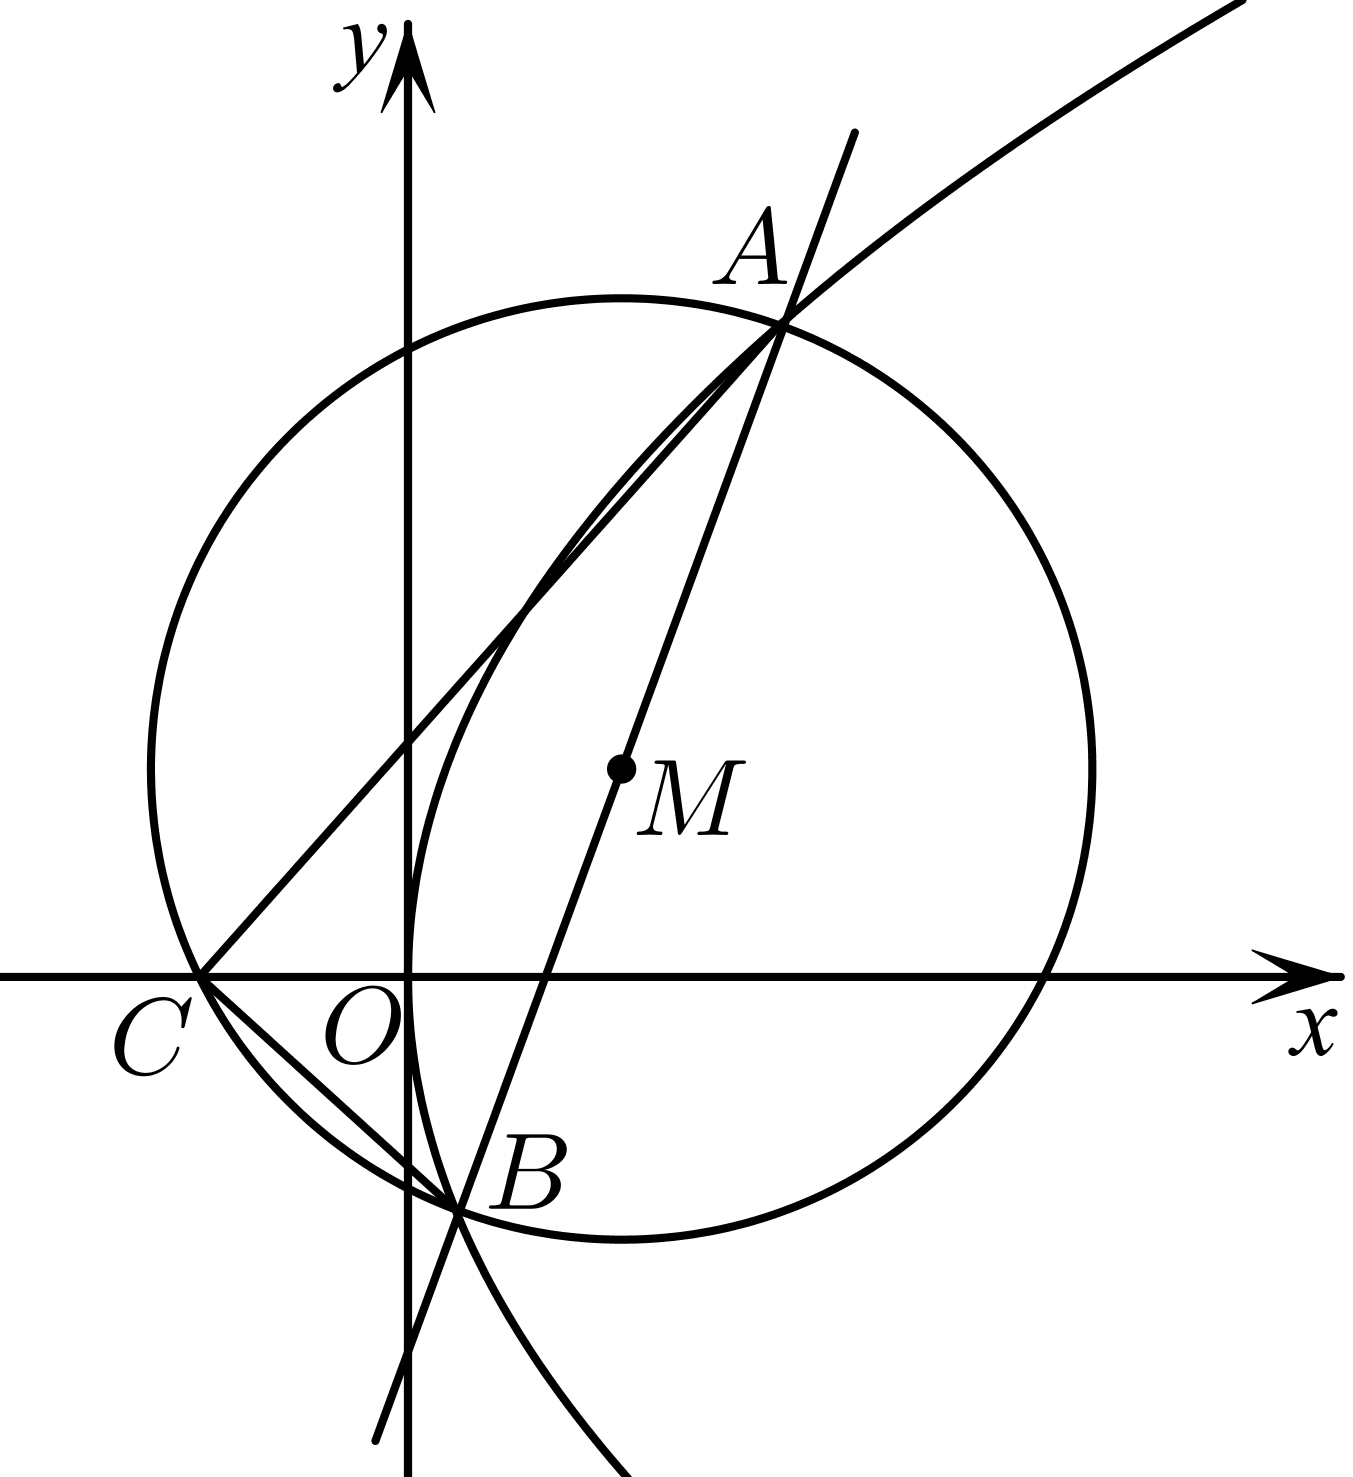
\includegraphics[width=38mm]{figs/18-12.png}}
\liubai[24mm]{解答书写区}

\begin{ansblock}[2章-练-课时18-12]
% ans:2章-练-课时18-12
\ansitem{12}{(1) y²=8x；(2) 存在，t=±√2/2}
\ansnote{详解}{(1) 设\(y^{2}=ax\)，准线\(x=-a/4=-2\)，得\(a=8\)，即\(y^{2}=8x\)。\par\noindent (2) 联立\(x=ty+1\)：\(y^{2}-8ty-8=0\)，得\(y_1+y_2=8t\)、\(y_1y_2=-8\)；\(x_1+x_2=t(y_1+y_2)+2=8t^{2}+2\)、\(x_1x_2=t^{2}y_1y_2+t(y_1+y_2)+1=1\)。设\(C(x_0,0)\)（\(x_0<0\)）。\(C\)在以\(AB\)为直径的圆上，即\(\angle ACB=90^{\circ}\)，\(\overrightarrow{CA}\cdot\overrightarrow{CB}=0\)：\((x_1-x_0)(x_2-x_0)+y_1y_2=0\)，即\(x_0^{2}-(8t^{2}+2)x_0+(x_1x_2+y_1y_2)=0\)，即\(x_0^{2}-(8t^{2}+2)x_0-7=0\)（\(*\)）。内心在\(x\)轴当且仅当\(x\)轴平分\(\angle ACB\)，即\(k_{CA}+k_{CB}=0\)：\(y_1(x_2-x_0)+y_2(x_1-x_0)=0\)，即\(2ty_1y_2+(y_1+y_2)(1-x_0)=0\)，即\(-16t+8t(1-x_0)=0\)，得\(8t(-1-x_0)=0\)。\(t=0\)时直线\(x=1\)垂直于\(x\)轴，与题设矛盾，舍；故\(x_0=-1\)（小于0，合题），代入（\(*\)）：\(1+(8t^{2}+2)-7=0\)，得\(t^{2}=1/2\)，即\(t=\pm\sqrt{2}/2\)。}
\end{ansblock}

\tihao{13}\zu{对称存在求直线×解答} \tieside{难(知识点一)}已知椭圆\(C\)：\(x^{2}/a^{2}+y^{2}/b^{2}=1\)（\(a>b>0\)）过点\((1,\sqrt{2}/2)\)，且焦距为2。(1) 求椭圆\(C\)的标准方程；(2) 设过点\(P(-2,0)\)的直线\(l\)与椭圆\(C\)交于不同的两点\(A\)、\(B\)，点\(G(0,-1/2)\)，如果\(|GA|=|GB|\)，求直线\(l\)的方程。
\liubai[24mm]{解答书写区}

\begin{ansblock}[2章-练-课时18-13]
% ans:2章-练-课时18-13
\ansitem{13}{(1) x²/2+y²=1；(2) y=(2−√2)/2·(x+2) 或 y=0}
\ansnote{详解}{(1) 焦距2，即\(c=1\)、\(a^{2}=b^{2}+1\)；点代入：\(1/a^{2}+(1/2)/b^{2}=1\)。令\(u=b^{2}\)：\(1/(u+1)+1/(2u)=1\)，即\(2u+(u+1)=2u(u+1)\)，\(2u^{2}-u-1=0\)，得\(u=1\)，即\(a^{2}=2\)、\(b^{2}=1\)，故\(x^{2}/2+y^{2}=1\)。\par\noindent (2) 先取\(y=0\)：\(A\)、\(B=(\pm\sqrt{2},0)\)，\(G\)在\(y\)轴上，\(|GA|=|GB|\)成立，是一解。\(k\neq 0\)时设\(l\)：\(y=k(x+2)\)，联立\(x^{2}+2y^{2}=2\)：\((1+2k^{2})x^{2}+8k^{2}x+8k^{2}-2=0\)，中点\(M\)：\(x_M=-4k^{2}/(1+2k^{2})\)、\(y_M=k(x_M+2)=2k/(1+2k^{2})\)。\(|GA|=|GB|\)当且仅当\(GM\perp l\)，即\(x_M+k(y_M+1/2)=0\)，两边乘\(2(1+2k^{2})\)：\(-8k^{2}+4k^{2}+k(1+2k^{2})=0\)，即\(k(2k^{2}-4k+1)=0\)（\(k\neq 0\)），得\(k=(2\pm\sqrt{2})/2\)。两交点条件：\(\Delta=8-16k^{2}>0\)，即\(k^{2}<1/2\)；\(k=(2+\sqrt{2})/2\)时\(k^{2}=(3+2\sqrt{2})/2>1/2\)，舍；\(k=(2-\sqrt{2})/2\)时\(k^{2}=(3-2\sqrt{2})/2<1/2\)，合题。故\(l\)：\(y=(2-\sqrt{2})/2\cdot(x+2)\)或\(y=0\)。}
\end{ansblock}

\tihao{14}\zu{拼接曲线综合×解答} \tieside{中档(知识点一)}如图，曲线\(C\)由上半椭圆\(C_1\)：\(y^{2}/a^{2}+x^{2}/b^{2}=1\)（\(a>b>0\)，\(y\geqslant 0\)）和部分抛物线\(C_2\)：\(y=-x^{2}+1\)（\(y\leqslant 0\)）连接而成，\(C_1\)与\(C_2\)的公共点为\(A\)、\(B\)，其中\(C_1\)的离心率为\(\sqrt{3}/2\)。(1) 求\(a\)、\(b\)的值；(2) 过点\(B\)的直线\(l\)与\(C_1\)、\(C_2\)分别交于点\(P\)、\(Q\)（均异于点\(A\)、\(B\)），是否存在直线\(l\)，使得以\(PQ\)为直径的圆恰好过点\(A\)？若存在，求出直线\(l\)的方程；若不存在，请说明理由。
\ansfig{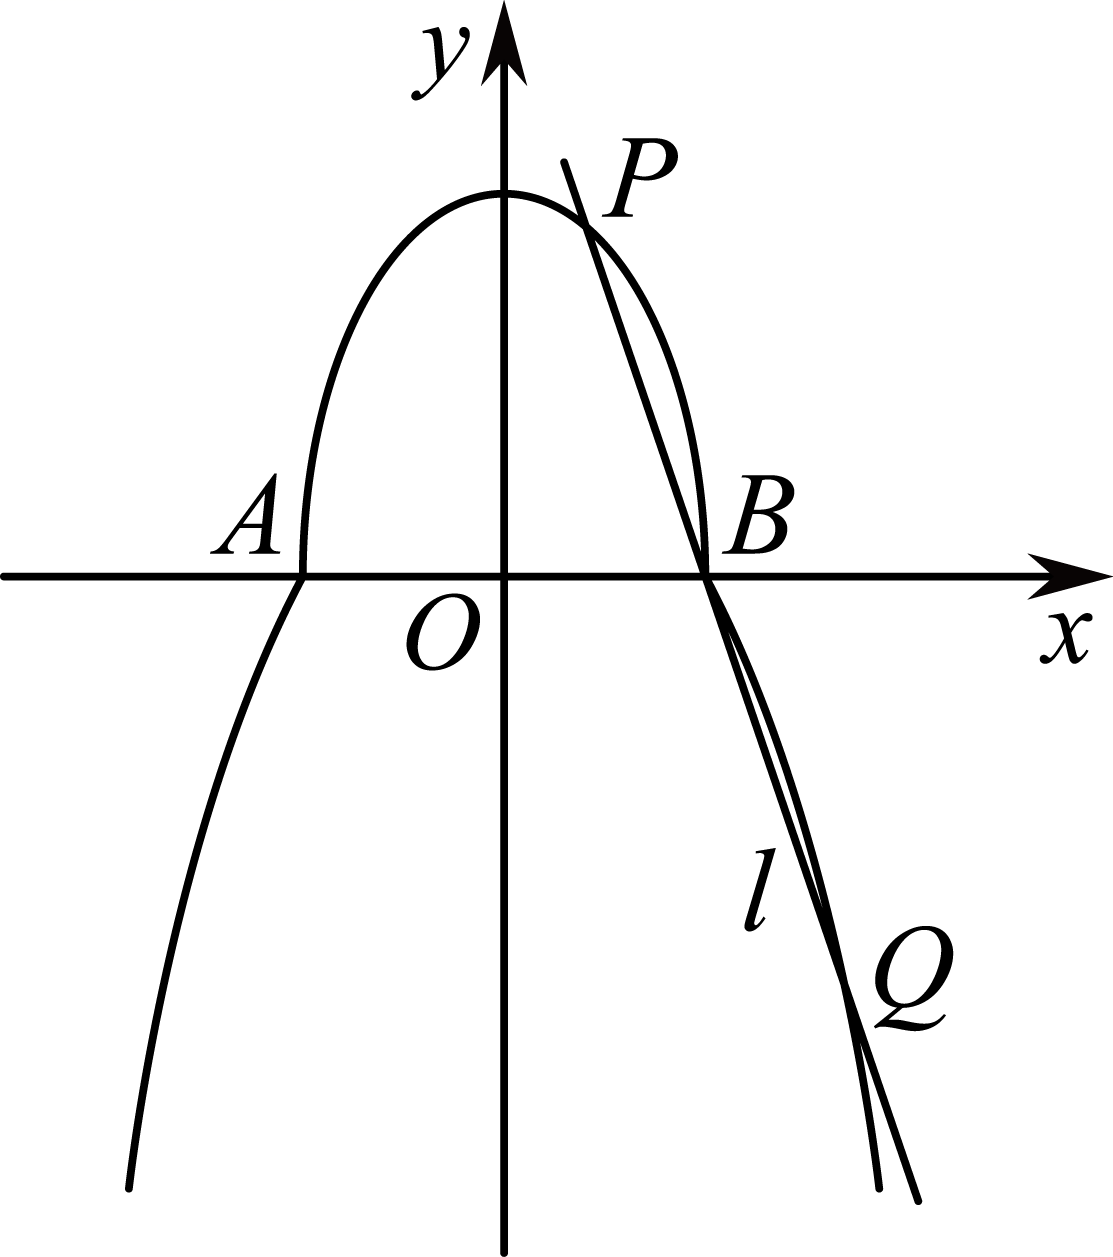
\includegraphics[width=38mm]{figs/18-14.png}}
\liubai[24mm]{解答书写区}

\begin{ansblock}[2章-练-课时18-14]
% ans:2章-练-课时18-14
\ansitem{14}{(1) a=2、b=1；(2) 存在，8x+3y−8=0}
\ansnote{详解}{(1) \(C_2\)与\(x\)轴交于\((\pm 1,0)\)，即\(A(-1,0)\)、\(B(1,0)\)，且\(x^{2}/b^{2}=1\)在\(y=0\)处，得\(b=1\)。\(e=c/a=\sqrt{3}/2\)，即\(c^{2}=3a^{2}/4\)；\(a^{2}-c^{2}=b^{2}=1\)，得\(a^{2}/4=1\)，即\(a=2\)。\par\noindent (2) \(C_1\)：\(y^{2}/4+x^{2}=1\)（\(y\geqslant 0\)）。设\(l\)：\(y=k(x-1)\)（\(k\neq 0\)；\(k=0\)时\(l\)与\(x\)轴重合，不合）。交\(C_1\)：\((k^{2}+4)x^{2}-2k^{2}x+k^{2}-4=0\)，一根\(x=1\)（点\(B\)），故\(x_P=(k^{2}-4)/(k^{2}+4)\)、\(y_P=k(x_P-1)=-8k/(k^{2}+4)\)。交\(C_2\)：\(k(x-1)=-(x-1)(x+1)\)，即\((x-1)(k+x+1)=0\)，得\(x_Q=-k-1\)（\(x_Q\neq 1\)，即\(k\neq -2\)）、\(y_Q=k(x_Q-1)=-k^{2}-2k\)。\par\noindent \(\overrightarrow{AP}=(2k^{2}/(k^{2}+4),-8k/(k^{2}+4))=(2k/(k^{2}+4))\cdot(k,-4)\)；\(\overrightarrow{AQ}=(-k,-k^{2}-2k)=-k(1,k+2)\)。以\(PQ\)为直径的圆过\(A\)当且仅当\(\overrightarrow{AP}\perp\overrightarrow{AQ}\)，即\(\overrightarrow{AP}\cdot\overrightarrow{AQ}=0\)，即\((2k/(k^{2}+4))\cdot(-k)\cdot[k-4(k+2)]=0\)，\(k\neq 0\)，得\(3k+8=0\)，即\(k=-8/3\)。回验落位：\(y_P=-8k/(k^{2}+4)=48/25>0\)（\(P\)在上半椭圆）、\(y_Q=-k^{2}-2k=-16/9\leqslant 0\)（\(Q\)在下半抛物线）。故存在\(l\)：\(y=-(8/3)(x-1)\)，即\(8x+3y-8=0\)。}
\end{ansblock}
% ============================================================
% 思维探索（题15~16＝18-15~16：解答2，居末档照库序）
% ============================================================
\dangbadge{思}{维}{探}{索}

\tihao{15}\zu{距离和最值×解答} \tieside{难(知识点三)}已知椭圆\(E\)：\(x^{2}/a^{2}+y^{2}/b^{2}=1\)（\(a>b>0\)）的左、右焦点分别为\(F_1\)、\(F_2\)，离心率为\(e=\sqrt{3}/2\)，过左焦点\(F_1\)作直线\(l_1\)交椭圆\(E\)于\(A\)、\(B\)两点，\(\triangle ABF_2\)的周长为8。(1) 求椭圆\(E\)的方程；(2) 若直线\(l_2\)：\(y=kx+m\)（\(km<0\)）与圆\(O\)：\(x^{2}+y^{2}=1\)相切，且与椭圆\(E\)交于\(M\)、\(N\)两点，\(|MF_2|+|NF_2|\)是否存在最小值？若存在，求出最小值和此时直线\(l_2\)的方程。
\liubai[24mm]{解答书写区}

\begin{ansblock}[2章-练-课时18-15]
% ans:2章-练-课时18-15
\ansitem{15}{(1) x²/4+y²=1；(2) 存在，min=2，此时 x−√2y−√3=0 或 x+√2y−√3=0}
\ansnote{详解}{(1) 周长\(=|AB|+|AF_2|+|BF_2|=4a=8\)，得\(a=2\)；\(e=\sqrt{3}/2\)，即\(c=\sqrt{3}\)、\(b^{2}=1\)，故\(x^{2}/4+y^{2}=1\)。\par\noindent (2) 相切，即\(d(O,l_2)=|m|/\sqrt{1+k^{2}}=1\)，得\(m^{2}=1+k^{2}\)。焦半径公式（\(|x_i|\leqslant 2\)保证非负）：\(|MF_2|=a-ex_M=2-(\sqrt{3}/2)x_M\)，同理\(|NF_2|=2-(\sqrt{3}/2)x_N\)，和\(=4-(\sqrt{3}/2)(x_M+x_N)\)。联立\(y=kx+m\)与\(x^{2}+4y^{2}=4\)：\((1+4k^{2})x^{2}+8kmx+4m^{2}-4=0\)，得\(x_M+x_N=-8km/(1+4k^{2})\)；\(km<0\)，即\(x_M+x_N=8\sqrt{k^{2}(1+k^{2})}/(1+4k^{2})\)。\par\noindent 设\(u=k^{2}>0\)，则\(x_M+x_N=8\sqrt{u(1+u)}/(1+4u)\)；对\(u(1+u)/(1+4u)^{2}\)求导，分子正比于\((1+2u)(1+4u)-8(u+u^{2})=1-2u\)，故\(u=1/2\)时最大，\(x_M+x_N\)的最大值为\(8\cdot(\sqrt{3}/2)/3=4\sqrt{3}/3\)，和的最小值为\(4-(\sqrt{3}/2)\cdot(4\sqrt{3}/3)=2\)。此时\(k^{2}=1/2\)、\(m^{2}=3/2\)且\(km<0\)，即\((k,m)=(\sqrt{2}/2,-\sqrt{6}/2)\)或\((-\sqrt{2}/2,\sqrt{6}/2)\)，即\(l_2\)：\(x-\sqrt{2}y-\sqrt{3}=0\)或\(x+\sqrt{2}y-\sqrt{3}=0\)。}
\end{ansblock}

\tihao{16}\zu{高难小题×解答} \tieside{难(知识点二)}设\(A\)、\(B\)为双曲线\(C\)：\(x^{2}/a^{2}-y^{2}/b^{2}=1\)（\(a>0\)，\(b>0\)）的左、右顶点，直线\(l\)过右焦点\(F\)且与双曲线\(C\)的右支交于\(M\)、\(N\)两点，当直线\(l\)垂直于\(x\)轴时，\(\triangle AMN\)为等腰直角三角形。(1) 求双曲线\(C\)的离心率；(2) 已知\(|AB|=4\)，若直线\(AM\)、\(AN\)分别交直线\(x=a/2\)于\(P\)、\(Q\)两点，当直线\(l\)的倾斜角变化时，以\(PQ\)为直径的圆是否过定点？若过定点，求出定点的坐标；若不过定点，请说明理由。
\liubai[24mm]{解答书写区}

\begin{ansblock}[2章-练-课时18-16]
% ans:2章-练-课时18-16
\ansitem{16}{(1) e=2；(2) 恒过定点 (4,0) 与 (−2,0)（两点同时在圆上）}
\ansnote{详解}{(1) \(l\perp x\)轴时\(M\)、\(N=(c,\pm b^{2}/a)\)；\(A\)在\(x\)轴上，\(|AM|=|AN|\)自动成立，故直角顶点只能是\(A\)（若直角在\(M\)，\(MA\)需水平，即\(y_M=0\)，不可能），即\(\angle MAN=90^{\circ}\)，\(k_{AM}=\pm 1\)，得\(b^{2}/a=a+c\)，即\(c^{2}-a^{2}=a^{2}+ac\)，\(e^{2}-e-2=0\)，得\(e=2\)（负根舍）。\par\noindent (2) \(2a=4\)，即\(a=2\)、\(c=2a=4\)、\(b^{2}=12\)，\(C\)：\(x^{2}/4-y^{2}/12=1\)，\(A(-2,0)\)、\(x=a/2=1\)。设\(l\)：\(x=ty+4\)（\(t\)为实数，\(t=0\)即\(l\perp x\)轴亦含；\(|t|<1/\sqrt{3}\)时与右支交两点）。代入得\((3t^{2}-1)y^{2}+24ty+36=0\)，得\(y_1y_2=36/(3t^{2}-1)\)、\(y_1+y_2=-24t/(3t^{2}-1)\)、\(x_1+x_2=t(y_1+y_2)+8=-8/(3t^{2}-1)\)、\(x_1x_2=t^{2}y_1y_2+4t(y_1+y_2)+16=(-12t^{2}-16)/(3t^{2}-1)\)。\par\noindent 直线\(AM\)过\(A(-2,0)\)、\(M(x_1,y_1)\)，在\(x=1\)处\(y=3y_1/(x_1+2)\)，即\(P(1,p)\)、\(Q(1,q)\)，其中\(p=3y_1/(x_1+2)\)、\(q=3y_2/(x_2+2)\)。而\((x_1+2)(x_2+2)=x_1x_2+2(x_1+x_2)+4=(-12t^{2}-16-16+12t^{2}-4)/(3t^{2}-1)=-36/(3t^{2}-1)\)，故\(pq=9y_1y_2/[(x_1+2)(x_2+2)]=9\cdot[36/(3t^{2}-1)]\cdot[(3t^{2}-1)/(-36)]=-9\)，与\(t\)无关。\par\noindent 以\(PQ\)为直径的圆：\((x-1)^{2}+(y-p)(y-q)=0\)，即\((x-1)^{2}+y^{2}-(p+q)y+pq=0\)。令\(y=0\)：\((x-1)^{2}=-pq=9\)，得\(x=4\)或\(x=-2\)——对每一条满足题设的\(l\)，\((4,0)\)与\((-2,0)\)同时在该圆上（源答案「或」字措辞不确：\(pq=-9\)使方程两根并立，非二选一）。特例回验：\(t=0\)时\(M\)、\(N=(4,\pm 6)\)，\(P(1,3)\)、\(Q(1,-3)\)，圆\((x-1)^{2}+y^{2}=9\)，两点均在圆上；\(3t^{2}-1=0\)时\(l\)平行渐近线仅一交点，不在题设内。}
\end{ansblock}

% ---- 尾块（\tailfill 置 \end{multicols} 前；无参＝内容尾随框，每件恰 1 处） ----
\tailfill

\end{multicols}
\end{document}
